\documentclass{standalone}
%
\usepackage{tikz}
\usetikzlibrary{backgrounds,bending,arrows.meta,shapes.callouts}
\usetikzlibrary{patterns}
\usepackage{tkz-euclide}
\usetkzobj{all}
\usepackage{xcolor}
%
\definecolor{space}{HTML}{1F2C4E}
\definecolor{mercury}{HTML}{846549}
\definecolor{venus}{HTML}{BB9765}
\definecolor{earth}{HTML}{0089FA}
\definecolor{mars}{HTML}{DC7B4E}
\definecolor{jupiter}{HTML}{A79476}
\definecolor{saturn}{HTML}{DBBD9B}
\definecolor{saturnring}{HTML}{857C73}
\definecolor{uranus}{HTML}{b1d8dd}
\definecolor{neptune}{HTML}{799bc1}
\definecolor{pluto}{HTML}{ceaa8a}
\definecolor{dida}{HTML}{FFDE00}
\definecolor{title}{HTML}{FBA706}
%
\usepackage{fontspec}
\setmainfont{Open Dyslexic}
%
\title{Viaggio verso la nube di Oort}
\begin{document}
	\tikzset{
		partial ellipse/.style args = {#1:#2:#3}{insert path={+ (#1:#3) arc (#1:#2:#3)}},
		notice/.style  = { draw, ellipse callout, callout relative pointer={#1} },
	}
	\begin{tikzpicture}[background rectangle/.style={fill=white},show background rectangle,>={[inset=0,angle'=27]Stealth}]
		\def\rsun{15}
		%
		\def\uam{0.387}
		\def\rmer{0.2}
		%
		\def\uav{0.723}
		\def\rven{0.5}
		%
		\def\uaet{1}
		\def\ret{0.53}
		%
		\def\uams{1.52}
		\def\rms{0.28}
		%
		\def\uaj{5.203}
		\def\rj{5.91}
		%
		\def\uasat{9.582}
		\def\rsat{4.98}
		%
		\def\uaur{19.191}
		\def\rur{2.11}
		%
		\def\uanp{30.069}
		\def\rnp{2.04}
		%
		\def\uap{39.48}
		\def\rp{0.1}
		%title
		\begin{scope}
			\draw [black,ultra thick,fill=title] (-15,4) rectangle (15,-3);
			\node at (0,2) {\textcolor{black}{\fontsize{90}{91}\selectfont Viaggio verso la}};
			\node at (0,-1) {\textcolor{black}{\fontsize{90}{91}\selectfont Nube di Oort}};
			%
			\draw [black,ultra thick,fill=dida] (5,-2.5) rectangle (14.8,-3.5);
			\node at (10,-3) {\textcolor{black}{\fontsize{20}{21}\selectfont 1 UA = 149597887.5 km}};
		\end{scope}
		%
		\begin{scope}[shift={(0,-8)}]
			\draw [ultra thick, fill=earth] (8.5,4) rectangle (13.5,-4);
			\node at (11,0) {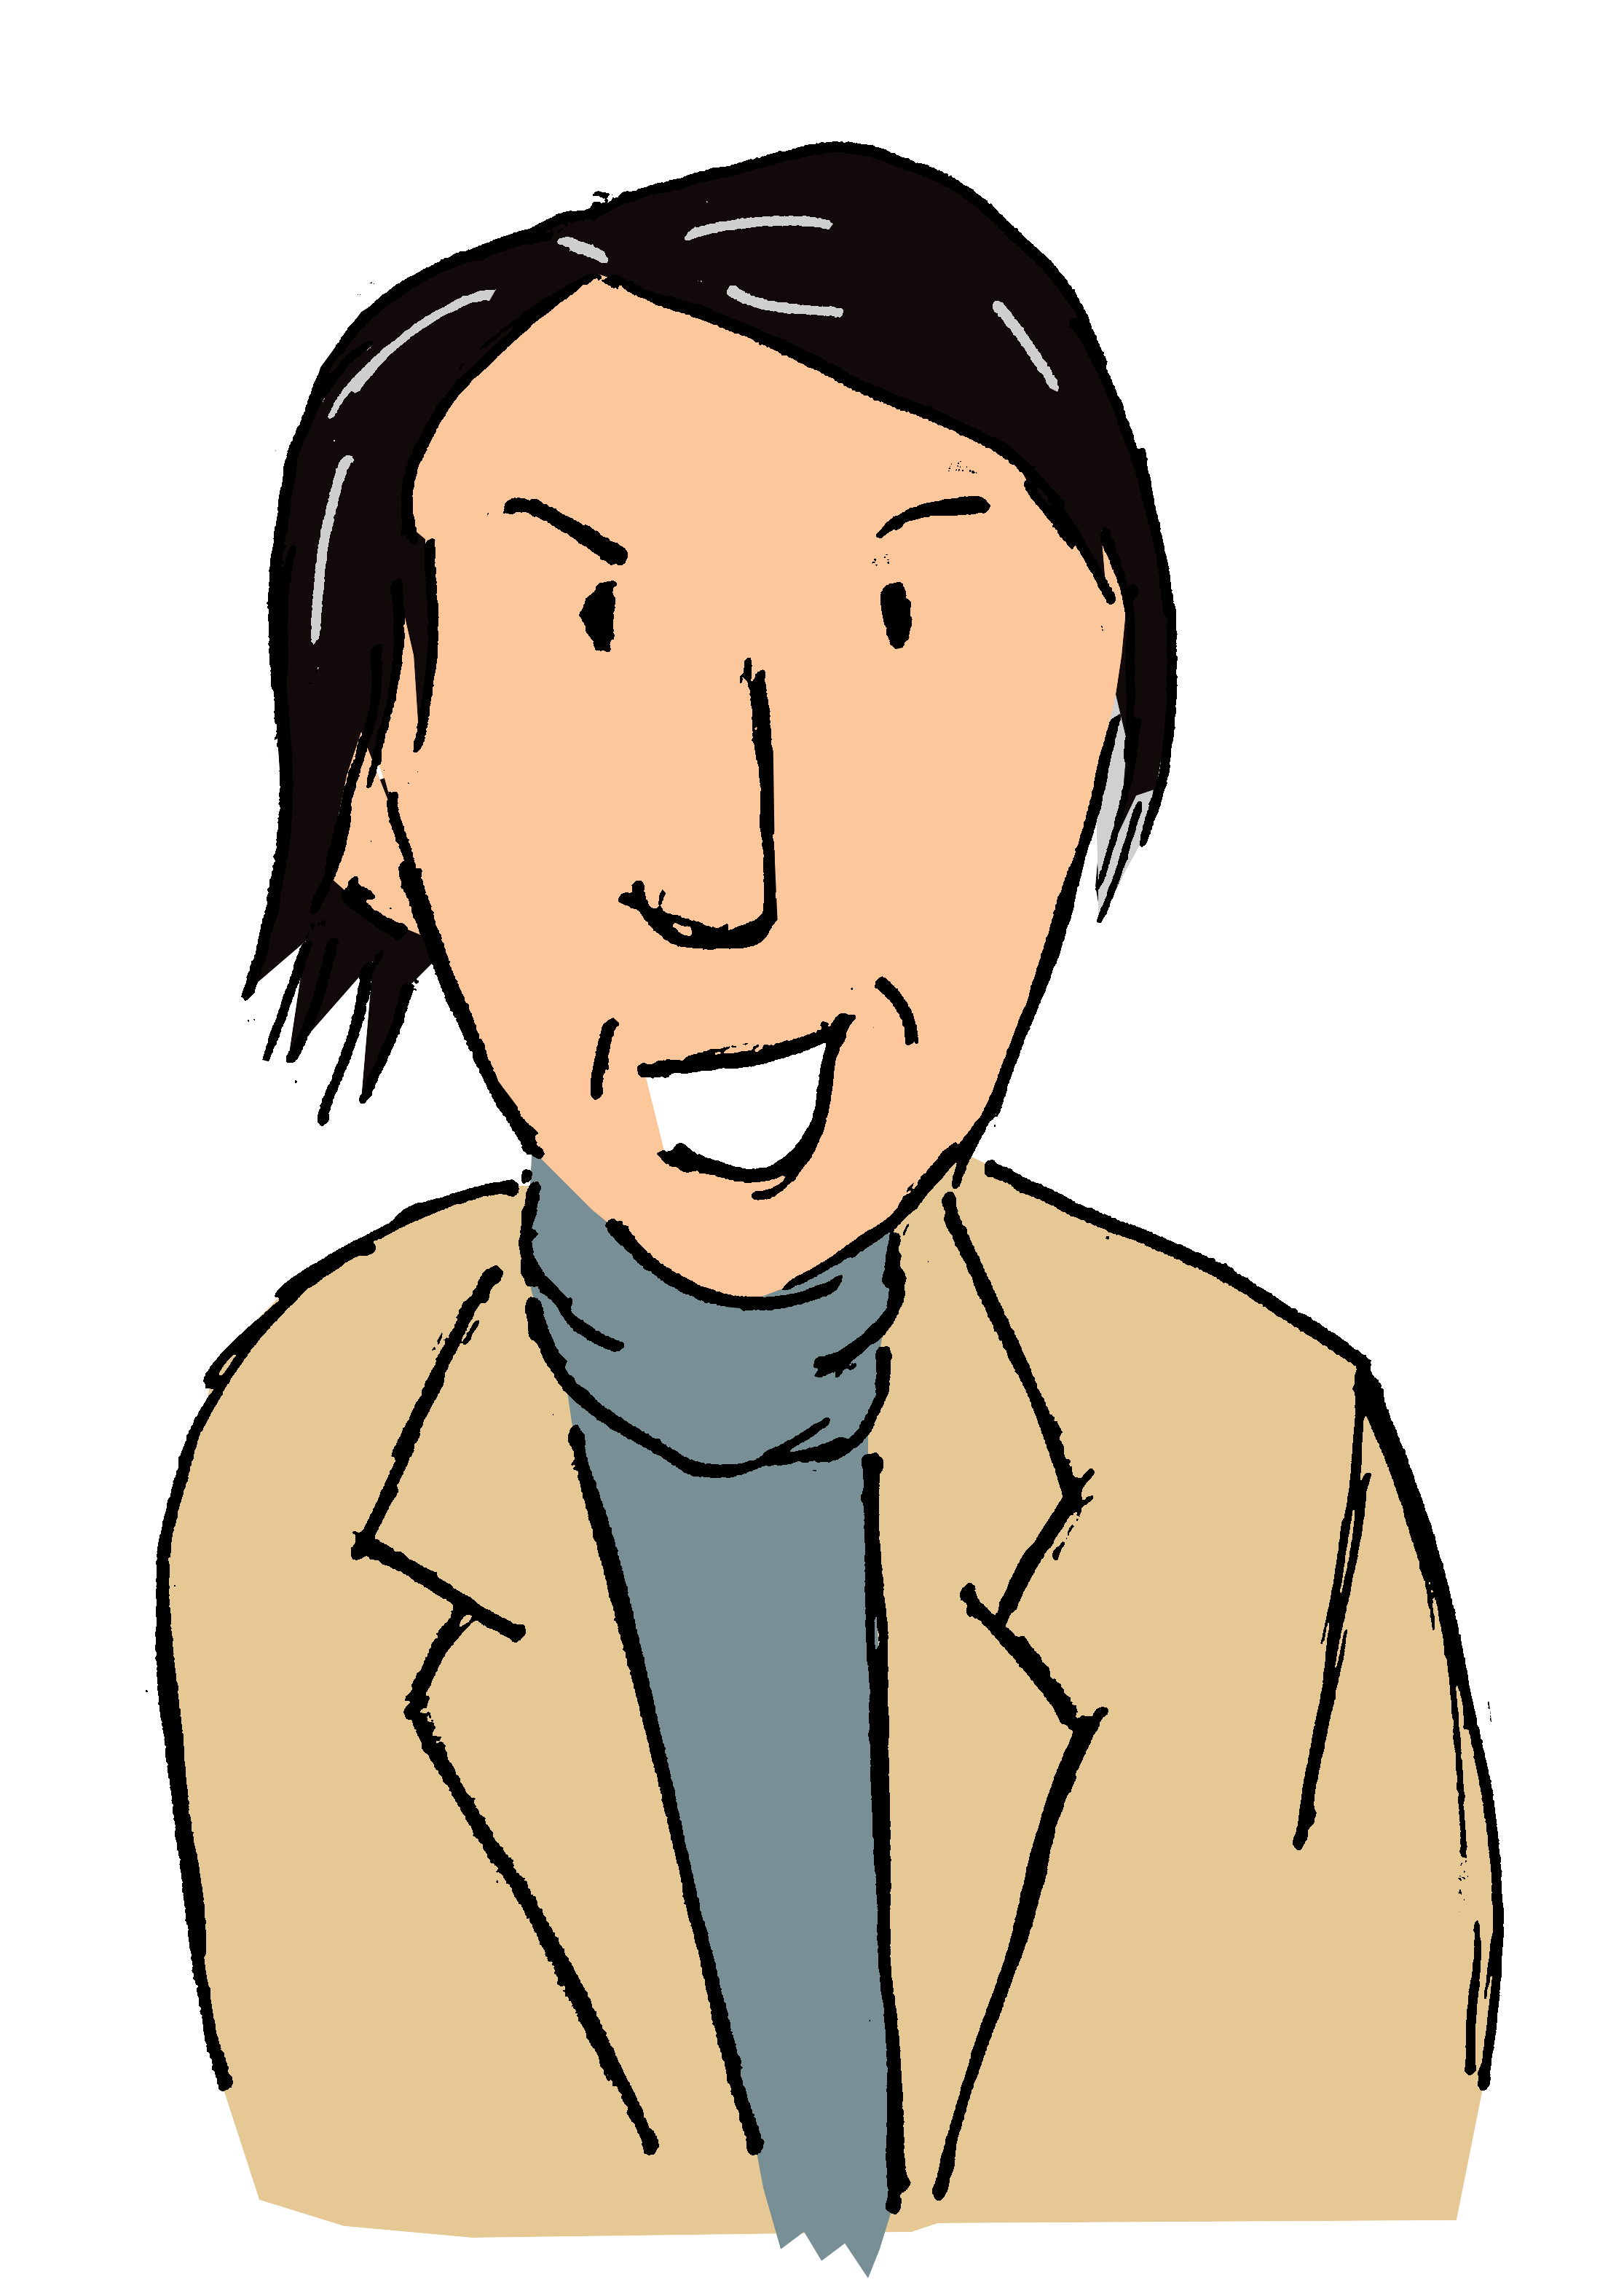
\includegraphics[width=5cm]{carl_sagan}};
			\node (example-textwidth-2) [notice={(3,0.5)}, ultra thick, right, align=center, text width=12cm, color=black, fill=white, font=\fontsize{23pt}{24pt}\selectfont] at (-11,-1) {Oggi facciamo un viaggio nel Sistema Solare verso la Nube di Oort, la culla delle comete!};
		\end{scope}
		% inner solar system
		\begin{scope}[shift={(-9,-20)}]
			\draw [fill=space,ultra thick] (6,6) rectangle (-6,-6);
			\tkzDefPoint(0,0){S}
			% asteroids
			\draw (S) [color=white,pattern=dots, pattern color=pluto,partial ellipse=0:360:3.28 and 3.28];
			\draw (S) [color=white,fill=space,partial ellipse=0:360:2.06 and 2.06];
			% mercury
			\draw (S) [color=white,partial ellipse=0:360:0.466 and 0.307];
			% venus
			\draw (S) [color=white,partial ellipse=0:360:0.728 and 0.718];
			% earth
			\draw (S) [color=white,partial ellipse=0:360:1.017 and 0.983];
			% mars
			\draw (S) [color=white,partial ellipse=0:360:1.666 and 1.382];
			% jupiter
			\draw (S) [color=white,partial ellipse=0:360:5.459 and 4.95];
			%
			\draw [fill=dida,ultra thick] (6.8,3.1) rectangle (25.2,-3.1);
			\node (example-textwidth-2) [right, align=left, text width=18cm, color=black, font=\fontsize{23pt}{24pt}\selectfont] at (7,0) {E' costituito dai pianeti compresi tra il Sole e l'orbita di Giove. Nell'ordine troviamo: Mercurio, Venere, Terra, Marte, la fascia principale degli asteroidi (la striscia circolare con i puntini) e, appunto, Giove.};
			%
			\draw [fill=earth!50!white,ultra thick] (7.2,4) rectangle (18.3,3);
			\node (example-textwidth-2) [right, align=left, text width=18cm, color=black, font=\fontsize{23pt}{24pt}\selectfont] at (7.5,3.5) {Il Sistema Solare interno};
			%
			\draw [<-,ultra thick, color=pluto] (-2.6,0) -- (-1.8,-5.5);
			\draw [fill=earth!50!white, ultra thick] (-2.5,-5) rectangle (7.5,-7);
			\node (example-textwidth-2) [right, align=left, text width=10cm, color=black, font=\fontsize{23pt}{24pt}\selectfont] at (-2.3,-6) {Fascia principale degli asteroidi};
		\end{scope}
		% outer solar system
		\begin{scope}[shift={(9,-35)}]
			\draw [fill=space,ultra thick] (6,6) rectangle (-6,-6);
			\begin{scope}[scale={(0.1)}]
				\tkzDefPoint(0,0){S}
				\tkzDefPoint(15,-15){P}
				% kuiper
				\draw (S) [color=white,pattern=dots, pattern color=pluto,partial ellipse=0:360:50 and 50];
				\draw (S) [color=white,fill=space,partial ellipse=0:360:30 and 30];
				% asteroids
				\draw (S) [color=white,pattern=dots, pattern color=pluto,partial ellipse=0:360:3.28 and 3.28];
				\draw (S) [color=white,fill=space,partial ellipse=0:360:2.06 and 2.06];
				% mercury
				\draw (S) [color=white,partial ellipse=0:360:0.466 and 0.307];
				% venus
				\draw (S) [color=white,partial ellipse=0:360:0.728 and 0.718];
				% earth
				\draw (S) [color=white,partial ellipse=0:360:1.017 and 0.983];
				% mars
				\draw (S) [color=white,partial ellipse=0:360:1.666 and 1.382];
				% jupiter
				\draw (S) [color=white,partial ellipse=0:360:5.459 and 4.95];
				% saturn
				\draw (S) [color=white,partial ellipse=0:360:10.12 and 9.04];
				% uranus
				\draw (S) [color=white,partial ellipse=0:360:20.1 and 18.29];
				% pluto
				\draw (P) [color=white,partial ellipse=0:360:39.48 and 38.24];
			\end{scope}
			%
			\draw [<-,ultra thick,color=pluto] (-2.8,-2.8) -- (-8,-5);
			\draw [fill=earth!50!white, ultra thick] (-10.1,-6) rectangle (-3.1,-5);
			\node (example-textwidth-2) [right, align=left, text width=10cm, color=black, font=\fontsize{23pt}{24pt}\selectfont] at (-10,-5.5) {Fascia di Kuiper};
			%
			\draw [fill=dida,ultra thick] (-25.2,3.1) rectangle (-6.6,-2.1);
			\node (example-textwidth-2) [right, align=left, text width=18cm, color=black, font=\fontsize{23pt}{24pt}\selectfont] at (-25,0.5) {E' costituito da tutti gli oggetti che si trovano oltre l'orbita di Giove. Nell'ordine troviamo: Saturno, Urano, Plutone e la fascia di Kuipert, costituita da asteroidi e pianeti nani.};
			%
			\draw [fill=earth!50!white,ultra thick] (-24.7,4) rectangle (-13.4,3);
			\node (example-textwidth-2) [right, align=left, text width=18cm, color=black, font=\fontsize{23pt}{24pt}\selectfont] at (-24.5,3.5) {Il Sistema Solare esterno};
		\end{scope}
		% sedna
		\begin{scope}[shift={(-9,-49)}]
			\draw [fill=space,ultra thick] (6,6) rectangle (-6,-6);
			\begin{scope}[scale={(0.1)},shift={(30,30)}]
				\tkzDefPoint(0,0){S}
				\tkzDefPoint(1.5,-1.5){P}
				\tkzDefPoint(-43.1,0){Sd}
				% kuiper
				\draw (S) [color=white,pattern=dots, pattern color=pluto,partial ellipse=0:360:5 and 5];
				\draw (S) [color=white,fill=space,partial ellipse=0:360:3 and 3];
				% jupiter
				\draw (S) [color=white,partial ellipse=0:360:0.5459 and 0.495];
				% saturn
				\draw (S) [color=white,partial ellipse=0:360:1.012 and 0.904];
				% uranus
				\draw (S) [color=white,partial ellipse=0:360:2.01 and 1.829];
				% pluto
				\draw (P) [color=white,partial ellipse=0:360:3.948 and 3.824];
				% sedna
				\draw (Sd) [color=white,rotate around={45:(S)},partial ellipse=0:360:50.6 and 26.7];
			\end{scope}
			%
			\draw [fill=dida,ultra thick] (6.8,3.1) rectangle (25.2,-3.1);
			\node (example-textwidth-2) [right, align=left, text width=18cm, color=black, font=\fontsize{23pt}{24pt}\selectfont] at (7,0) {90377 Sedna è un pianeta nano che orbita oltre l'orbita di Nettuno e la fascia di Kuiper. Ha un'orbita particolarmente eccentrica che varia tra un perielio vicino al sistema solare esterno, e un afelio di ben 5 giorni luce dal Sole.};
			%
			\draw [fill=earth!50!white,ultra thick] (7.2,4) rectangle (18.3,3);
			\node (example-textwidth-2) [right, align=left, text width=18cm, color=black, font=\fontsize{23pt}{24pt}\selectfont] at (7.5,3.5) {Sedna};
		\end{scope}
		% oort cloud
		\begin{scope}[shift={(9,-62)}]
			\draw [fill=space,ultra thick] (6,6) rectangle (-6,-6);
			\draw [pattern=dots, pattern color=pluto] (6,6) rectangle (-6,-6);
			\begin{scope}[scale={(0.1)},shift={(30,30)}]
				%oort
				\draw (0,0) [color=white,fill=space,partial ellipse=0:360:21 and 21];
				% uranus
				\draw (0,0) [color=white,partial ellipse=0:360:0.201 and 0.1829];
				% pluto
				\draw (0,0) [color=white,partial ellipse=0:360:0.3948 and 0.3824];
				% sedna
				\draw (-4.31,0) [color=white,rotate around={45:(0,0)},partial ellipse=0:360:5.06 and 2.67];
			\end{scope}
			%
			\draw [fill=dida,ultra thick] (-25.2,3.1) rectangle (-6.6,-2.1);
			\node (example-textwidth-2) [right, align=left, text width=18cm, color=black, font=\fontsize{23pt}{24pt}\selectfont] at (-25,0.5) {E' una nube sferica posta tra le 20000 e le 100000 UA dal Sole. In realtà non è mai stata osservata. La sua esistenza è stata teorizzata da Jan Oort come luogo d'origine delle comete.};
			%
			\draw [fill=earth!50!white,ultra thick] (-24.7,4) rectangle (-18.9,3);
			\node (example-textwidth-2) [right, align=left, text width=18cm, color=black, font=\fontsize{23pt}{24pt}\selectfont] at (-24.5,3.5) {Nube di Oort};
		\end{scope}
		%
		\begin{scope}[shift={(0,-73)}]
			\node at (-10,0) {
\includegraphics[width=8cm]{jan_oort}};
			\node (example-textwidth-2) [notice={(-3,0.5)}, ultra thick, right, align=center, text width=12cm, color=black, fill=white, font=\fontsize{23pt}{24pt}\selectfont] at (-6,-1) {Se le comete fossero nate insieme con il Sistema Solare, allora oggi non ne avremmo dovuto osservare nessuna: il loro nucleo viene distrutto dopo numerosi passaggi accanto al Sole.};
			\node at (9,-10) {
\includegraphics[width=8cm]{jan_oort}};
			\node (example-textwidth-2) [notice={(3,0.5)}, ultra thick, right, align=center, text width=12cm, color=black, fill=white, font=\fontsize{23pt}{24pt}\selectfont] at (-13,-11) {Per cui l'unica possibilità per spiegare come mai le continuiamo a osservare ancora oggi è che esse vengono originate in una zona posta ai confini del Sistema Solare.};
		\end{scope}
		%
		\begin{scope}[shift={(0,-93)}]
			\draw [ultra thick, fill=earth] (-12.5,4) rectangle (-7.5,-4);
			\node at (-10,0) {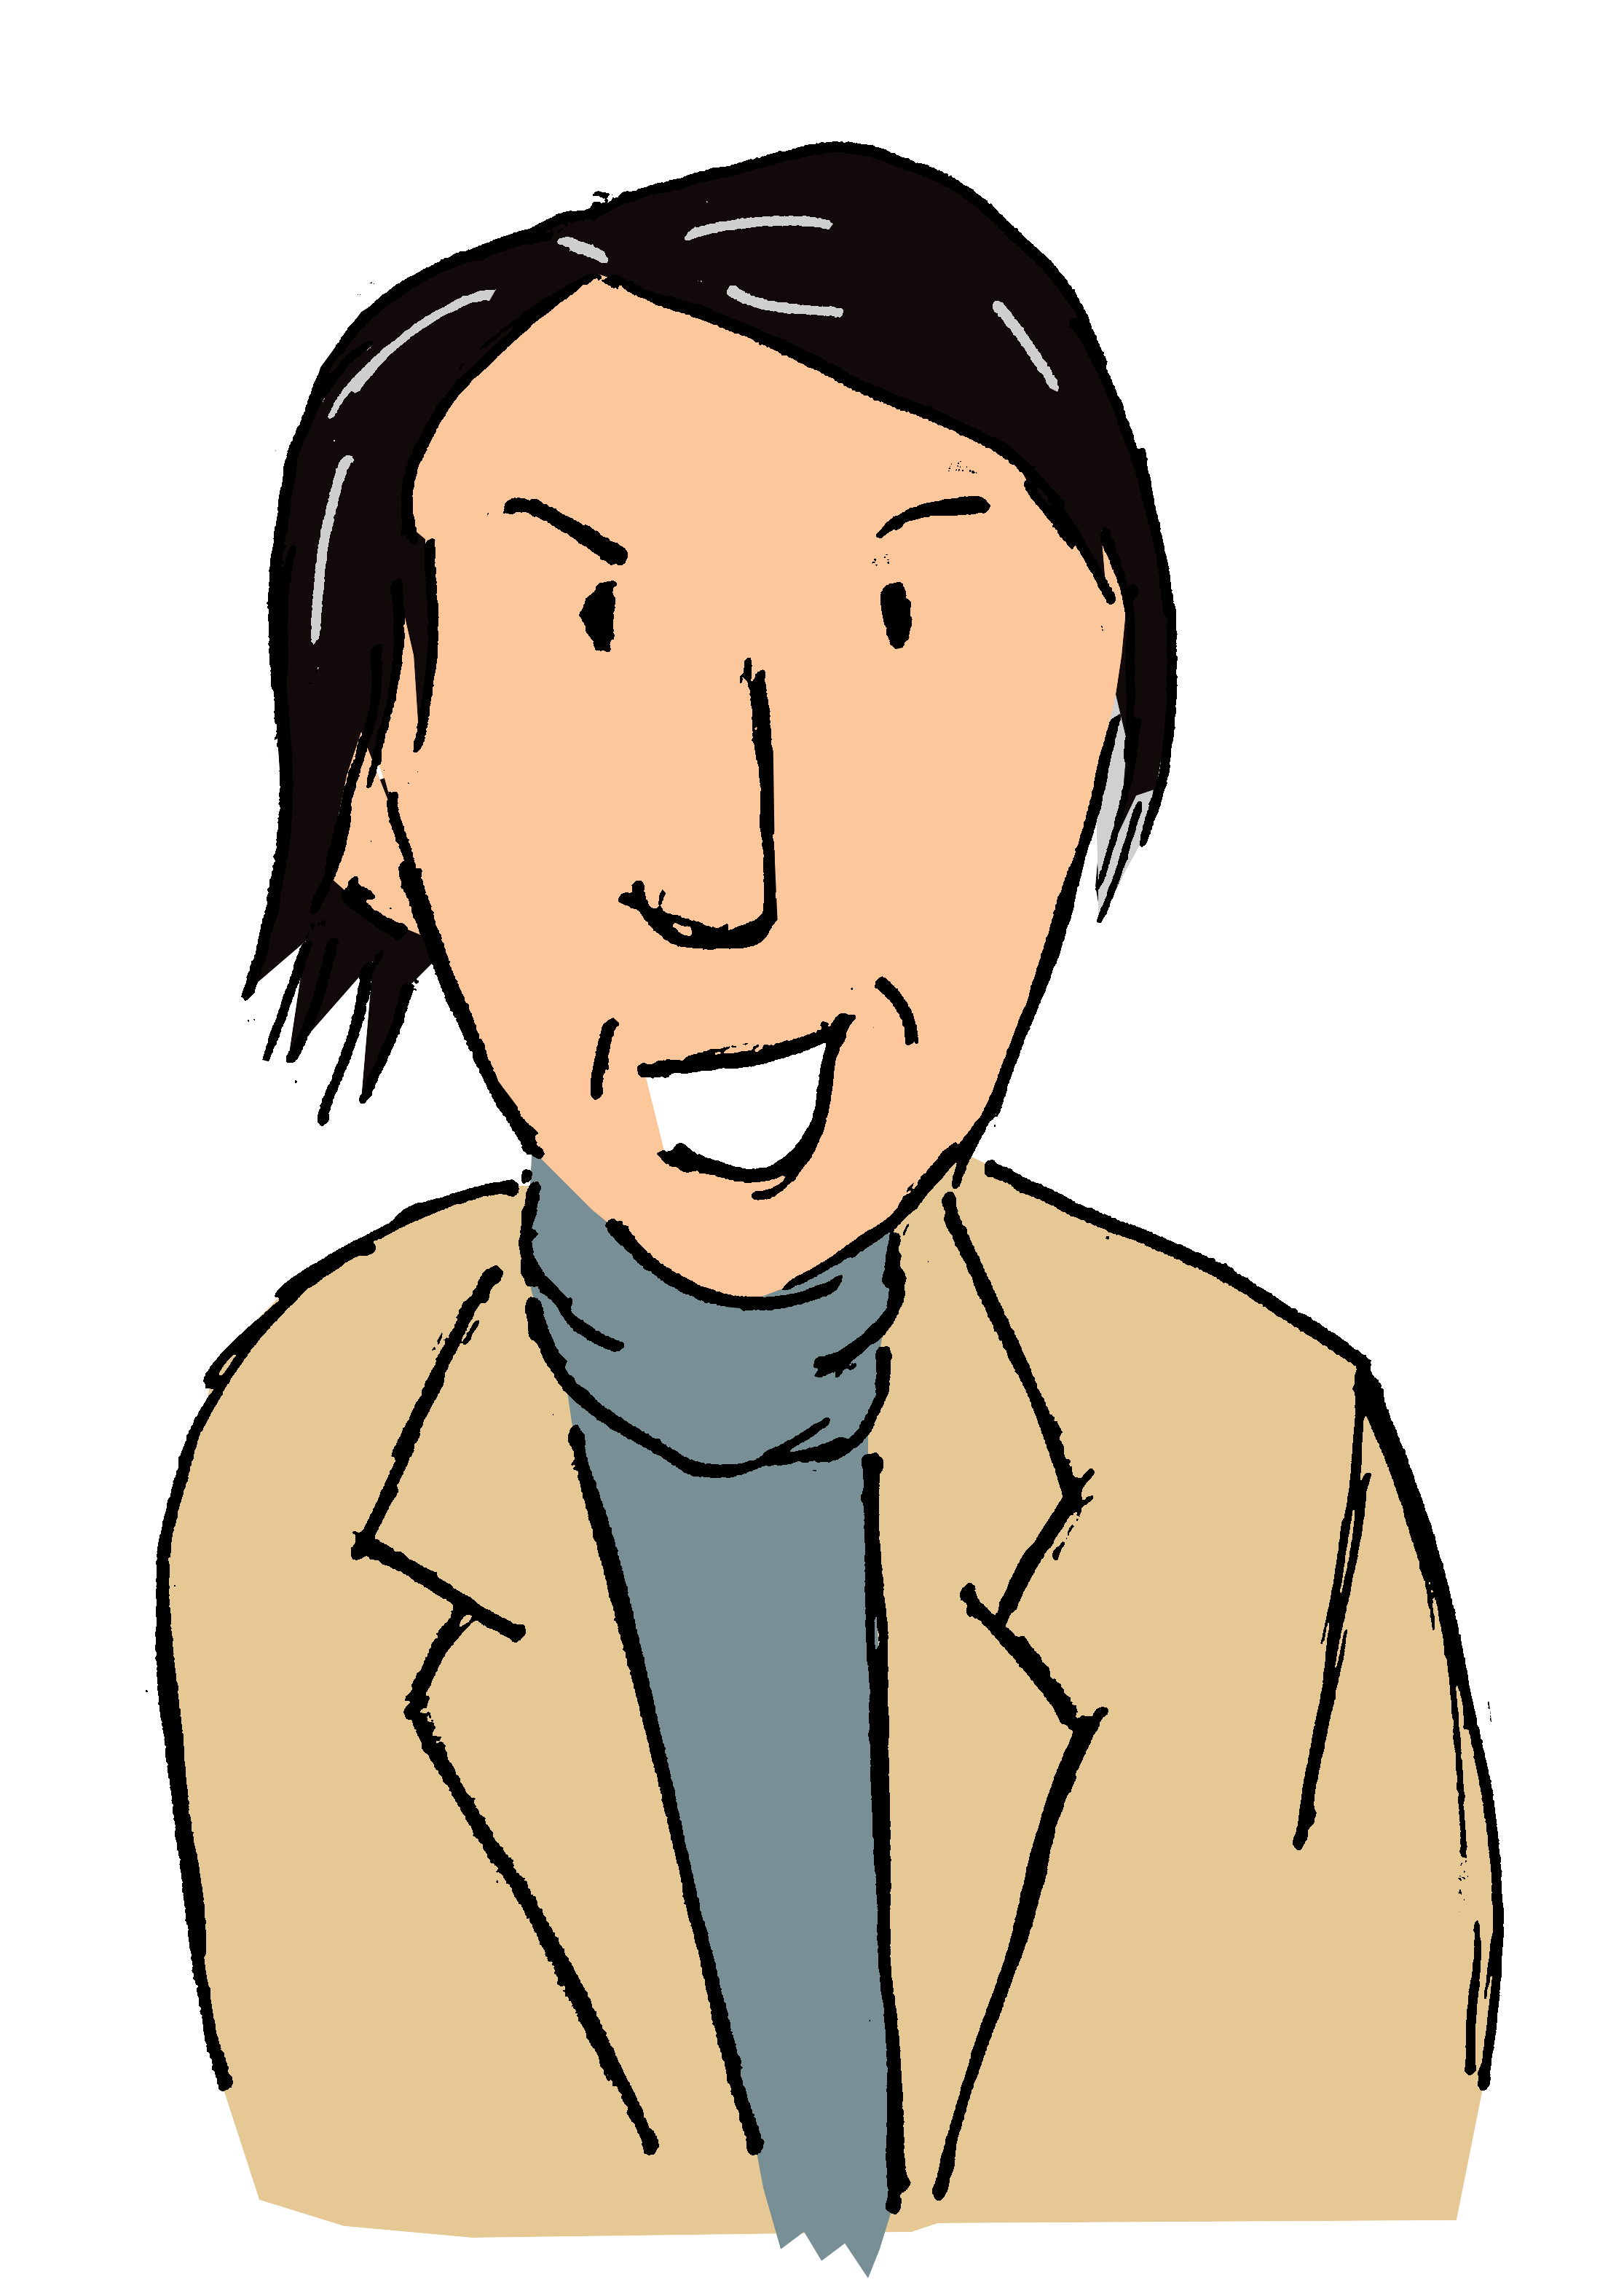
\includegraphics[width=5cm]{carl_sagan}};
			\node (example-textwidth-2) [notice={(-3,0.5)}, ultra thick, right, align=center, text width=14cm, color=black, fill=white, font=\fontsize{23pt}{24pt}\selectfont] at (-6,-1) {Si racconta che Oort sia stato uno dei pochi a poter osservare la cometa di Halley in vita in due occasioni. La prima volta quando aveva 10 anni, insieme con il padre, nei pressi di Noordwijk, in Olanda. La seconda volta 76 anni dopo, nel 1986.};
		\end{scope}
		%
		\begin{scope}[shift={(0,-100)}]
			\node at (12,0) () {
\includegraphics[width=3.7cm]{licenza}};
			\node[left] at (10,0) {\textcolor{black}{\fontsize{14}{15}\selectfont Testi e grafica: @ulaulaman - Gianluigi Filippelli}};
		\end{scope}
	\end{tikzpicture}
%
\end{document}
